%This is the fourth chapter of the dissertation

%The following command starts your chapter. If you want different titles used in your ToC and at the top of the page throughout the chapter, you can specify those values here. Since Columbia doesn't want extra information in the headers and footers, the "Top of Page Title" value won't actually appear.

\pagestyle{cu}
\graphicspath{{./Chapter4/images/}}

\chapter[Measuring the Low Energy Light and Charge Yield of Nuclear Recoils in Liquid Xenon][Measuring the Low Energy Light and Charge Yield of Nuclear Recoils in Liquid Xenon]{Measuring the Low Energy Light and Charge Yield of Nuclear Recoils in Liquid Xenon}
\label{chap:nerix}

%As was discussed in the second and third chapter of this work, understanding the response of liquid xenon to nuclear recoils is very important for the dark matter search as many candidates, including WIMPs, are expected to interact with atomic nuclei.  Liquid xenon detectors continue to grow in size yet this only makes their calibration, specifically with regards to nuclear recoils, increasingly difficult.  

As was discussed in the previous chapters, dual-phase liquid xenon TPCs lead the search for WIMPs.  These detectors continue to grow in size and reduce their background making them increasingly more sensitive to dark matter.  As mentioned in the previous chapter, XENON1T is the largest and most sensitive of these detectors with a total mass of 3,200 kg of liquid xenon \cite{aprile2017first}.  Since WIMPs are expected to interact primarily with atomic nuclei and the differential scattering rate of WIMPs and Standard Model particles are generally expected to increase with decreasing interaction energy, it is crucial to understand the properties of nuclear recoils in LXe down to the few keV energy scale.  

While larger detector sizes (in the form of larger fiducial volumes) make WIMP searches more and more sensitive, they do come with a drawback: calibrations, especially calibrations with external sources, becoming significantly more difficult.   However, understanding the signal output by a LXe TPC can essentially be broken down into two steps: the actual light and charge production and the detector physics.  While the detector physics is unique for each detector used and therefore must be measured for each one, the light and charge production mechanisms are only unique to the medium.  Therefore, if we can effectively decouple the two steps, we can measure the light and charge production mechanism in a detector optimized for calibrations and use it in other detectors.  

As LXe detectors have scaled in size, several of these optimized detectors have been built for exactly this purpose: to measure the light and charge production of liquid xenon to electronic and nuclear recoils.  While each of these detectors was slightly different and designed for a specific purpose, they shared the same relatively simple operating procedure: measure the light and charge produced from an interaction of a known type (electronic or nuclear recoil) and energy.  The neriX (Nuclear and Electronic Recoils in xenon) detector at Columbia University is one of these optimized detectors and has already successfully provided the most precise measurements of the light and charge yield of liquid xenon at multiple electric fields.  In this chapter, we will discuss the measurement of the light and charge yield of low energy nuclear recoils in liquid xenon using the neriX detector at Columbia University.

\section{Experimental Setup}
\label{sec:nerix_expt_setup}

In chapter three, we discussed the nuclear recoil calibration of XENON1T.  In this calibration, an americium-beryllium (AmBe) source was used to irradiate the liquid xenon inside of the detector with MeV energy neutrons.  Simulation is performed to determine the energy spectrum of single scatters in the detectors but, for the most part, the spectrum is defined by the relative cross-section of elastic scatters at different energies ultimately resulting in an exponentially falling energy spectrum as seen in \figref{fig:xe1t_nr_energy_spec}.  In this calibration setup, the energy of each individual event is unknown and at the end of the day are using the entire energy spectrum to match our data.  While this can be an effective way to measure the response of liquid xenon to nuclear recoils, it proves to be very difficult in practice with such a featureless energy spectrum.  This type of measurement where one compares an energy spectrum to data is typically referred to as an \textit{indirect} measurement and has been used successfully to measure the light and charge production process of electronic and nuclear recoils \cite{aprile2013response, akerib2016tritium, aprile2017tritium}.

Measurements in neriX and other smaller, calibration optimized detectors follow a different approach.  A monoenergetic source is used to irradiate the detector where the incoming particle will scatter a single time before scattering into a secondary detector.  For electronic recoils, the secondary detector can be a high-purity germanium detector or sodium-iodide detector with an excellent energy resolution.  When this is the case, assuming the incoming radiation did not scatter with other materials around the detector, the energy of the interaction is known very precisely.  Unfortunately when measuring the response of liquid xenon to nuclear recoils in these detectors, no equivalent secondary detectors exist that will precisely measure the energy of the incoming neutron.  Instead we can use the position of the secondary detector as a proxy for the energy since the energy transferred to a xenon nucleus by a neutron is completely determined by the scattering angle.  This relationship between the energy of the recoiling nucleus and the angle is shown for non-relativistic neutron energies in \eqnref{eqn:nerix_energy_scattering_angle} where $m_n$ is the mass of the neutron, $m_{\textrm{Xe}}$ is the mass of the xenon nucleus, $E_r$ is the energy of the recoiling nucleus, $E_n$ is the energy of the incoming neutron, and $\theta$ is the scattering angle \cite{knoll2010radiation}.

\begin{equation}
        \label{eqn:nerix_energy_scattering_angle}
        E_r \approx E_n \frac{2 m_n m_{\textrm{Xe}}}{(m_n + m_{\textrm{Xe}})^2}(1 - \textrm{cos} \theta)
\end{equation}

A schematic of the experimental setup for neriX using this \textit{fixed-angle} technique is shown in \figref{fig:nerix_expt_schematic}.  The neutron source in this measurement was a \ce{^2H}$(d, n)$\ce{^3He} generator provided by the Schlumberger Princeton Technology Center which produces 2.45 MeV neutrons at an angle of $\frac{\pi}{2}$.  The secondary detectors used were Eljen Technologies M510 detectors filled with the EJ301 liquid scintillator, chosen for their excellent pulse shape discrimination.  


\begin{figure}[t]
        \centering
	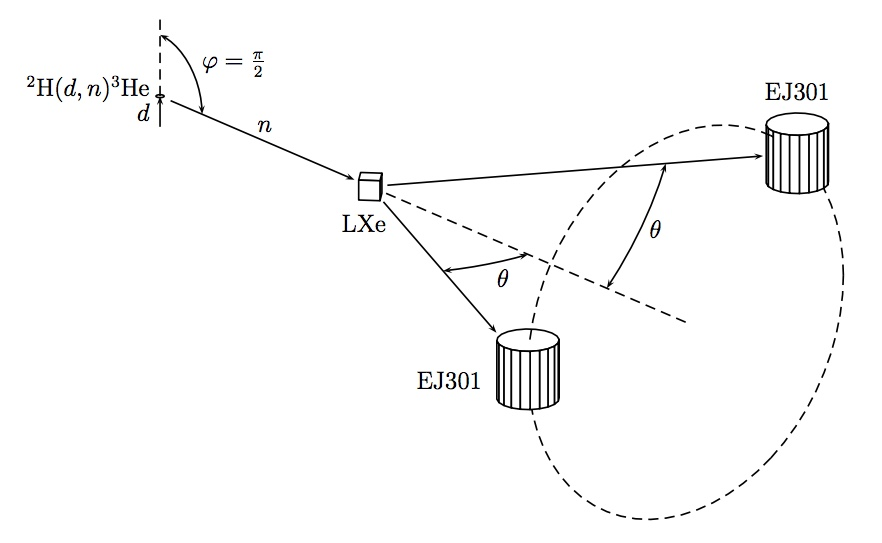
\includegraphics[width=0.9\textwidth]{nerix_expt_schematic}
	\caption{A schematic for the experimental setup used in this measurement of the light and charge yields for nuclear recoils.  2.45 MeV neutrons are produced at an angle of $\frac{\pi}{2}$ in the neutron generator.  Some of these neutrons scatter a single time in the liquid xenon and then deposit some of their energy in the EJ301 liquid scintillator for discrimination versus background.  Image Credit: \citeref{plante2011new}.}
	\label{fig:nerix_expt_schematic}
\end{figure}


\begin{figure}[bt]
        \centering
	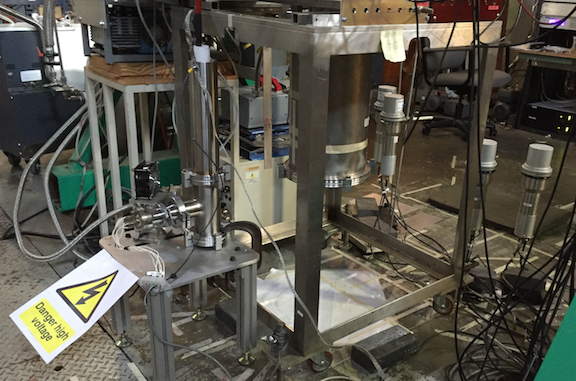
\includegraphics[width=0.9\textwidth]{nerix_experimental_setup}
	\caption{A photo of the fixed-angle setup with the neriX detector.  On the left is our neutron generator inside of its stainless stell case.  In the center is the outer portion of the cryostat and on the right are four of the M510 liquid scintillator detectors.}
	\label{fig:nerix_experimental_setup}
\end{figure}



\subsection{neriX Detector}

In this section we will discuss the neriX detector.  neriX was specifically designed to minimize the amount of inactive xenon and materials surrounding the TPC to minimize undetectable energy depositions and with electronics such that it can systematically scan electric fields ranging from approximately 0.15 V/cm to 2.5 kV/cm in the LXe.  These features make neriX an ideal detector for measuring the low-energy response of electronic and nuclear recoils at electric fields relevant to the dark matter search.

For more details on the design and construction of neriX, please refer to chapters four and five of \citeref{goetzke2015low}.

\subsubsection{TPC}

The neriX TPC (shown in \figref{fig:nerix_tpc_labeled}), like XENON1T, was also constructed with PTFE (teflon).  The teflon pieces in neriX are stackable and compressed by stainless steel springs.  The TPC at liquid xenon temperature has an inner diameter of 43 mm.  neriX also included four stainless steel hexagonal meshes and a single field shaping ring to control the electric fields inside of the TPC.  The cathode (used to produce the drift field inside the liquid xenon), the gate (kept at ground near the liquid surface), and the anode (used to extract electrons from the liquid surface and into the gas) were each made of  125 $\mu$m thick wires and 3 mm pitch (distance between parallel wire segments).  A photo of the gate mesh from above is shown in \figref{fig:nerix_tpc_mesh}.  The final mesh was a screening mesh (labeled the ``bottom grid'' in \figref{fig:nerix_tpc_labeled}) used to shield the bottom PMT and was also made a 3 mm pitch but with 25 $\mu$m thick wires (to reduce its surface area).  The field shaping ring is simply a copper coaxial wire embedded in the teflon wall of the TPC 7 mm above the cathode.  The location of the shaping ring was to maximize uniformity of the drift field at an electric field of 1 kV/cm.  The distance between the cathode and the gate mesh, the maximum drift distance of electrons in the TPC, was 23.4 mm.


\begin{figure}[t]
        \centering
	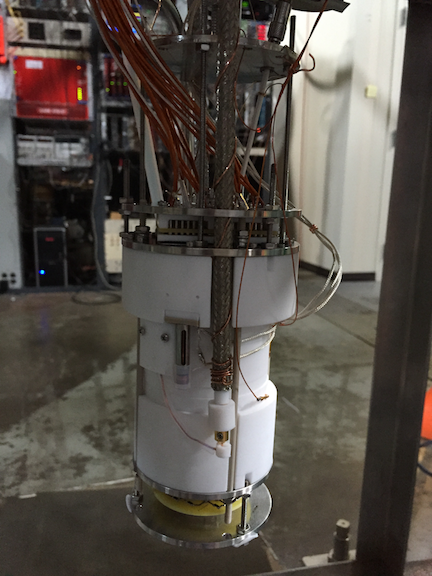
\includegraphics[width=0.50\textwidth]{nerix_tpc_anode}
	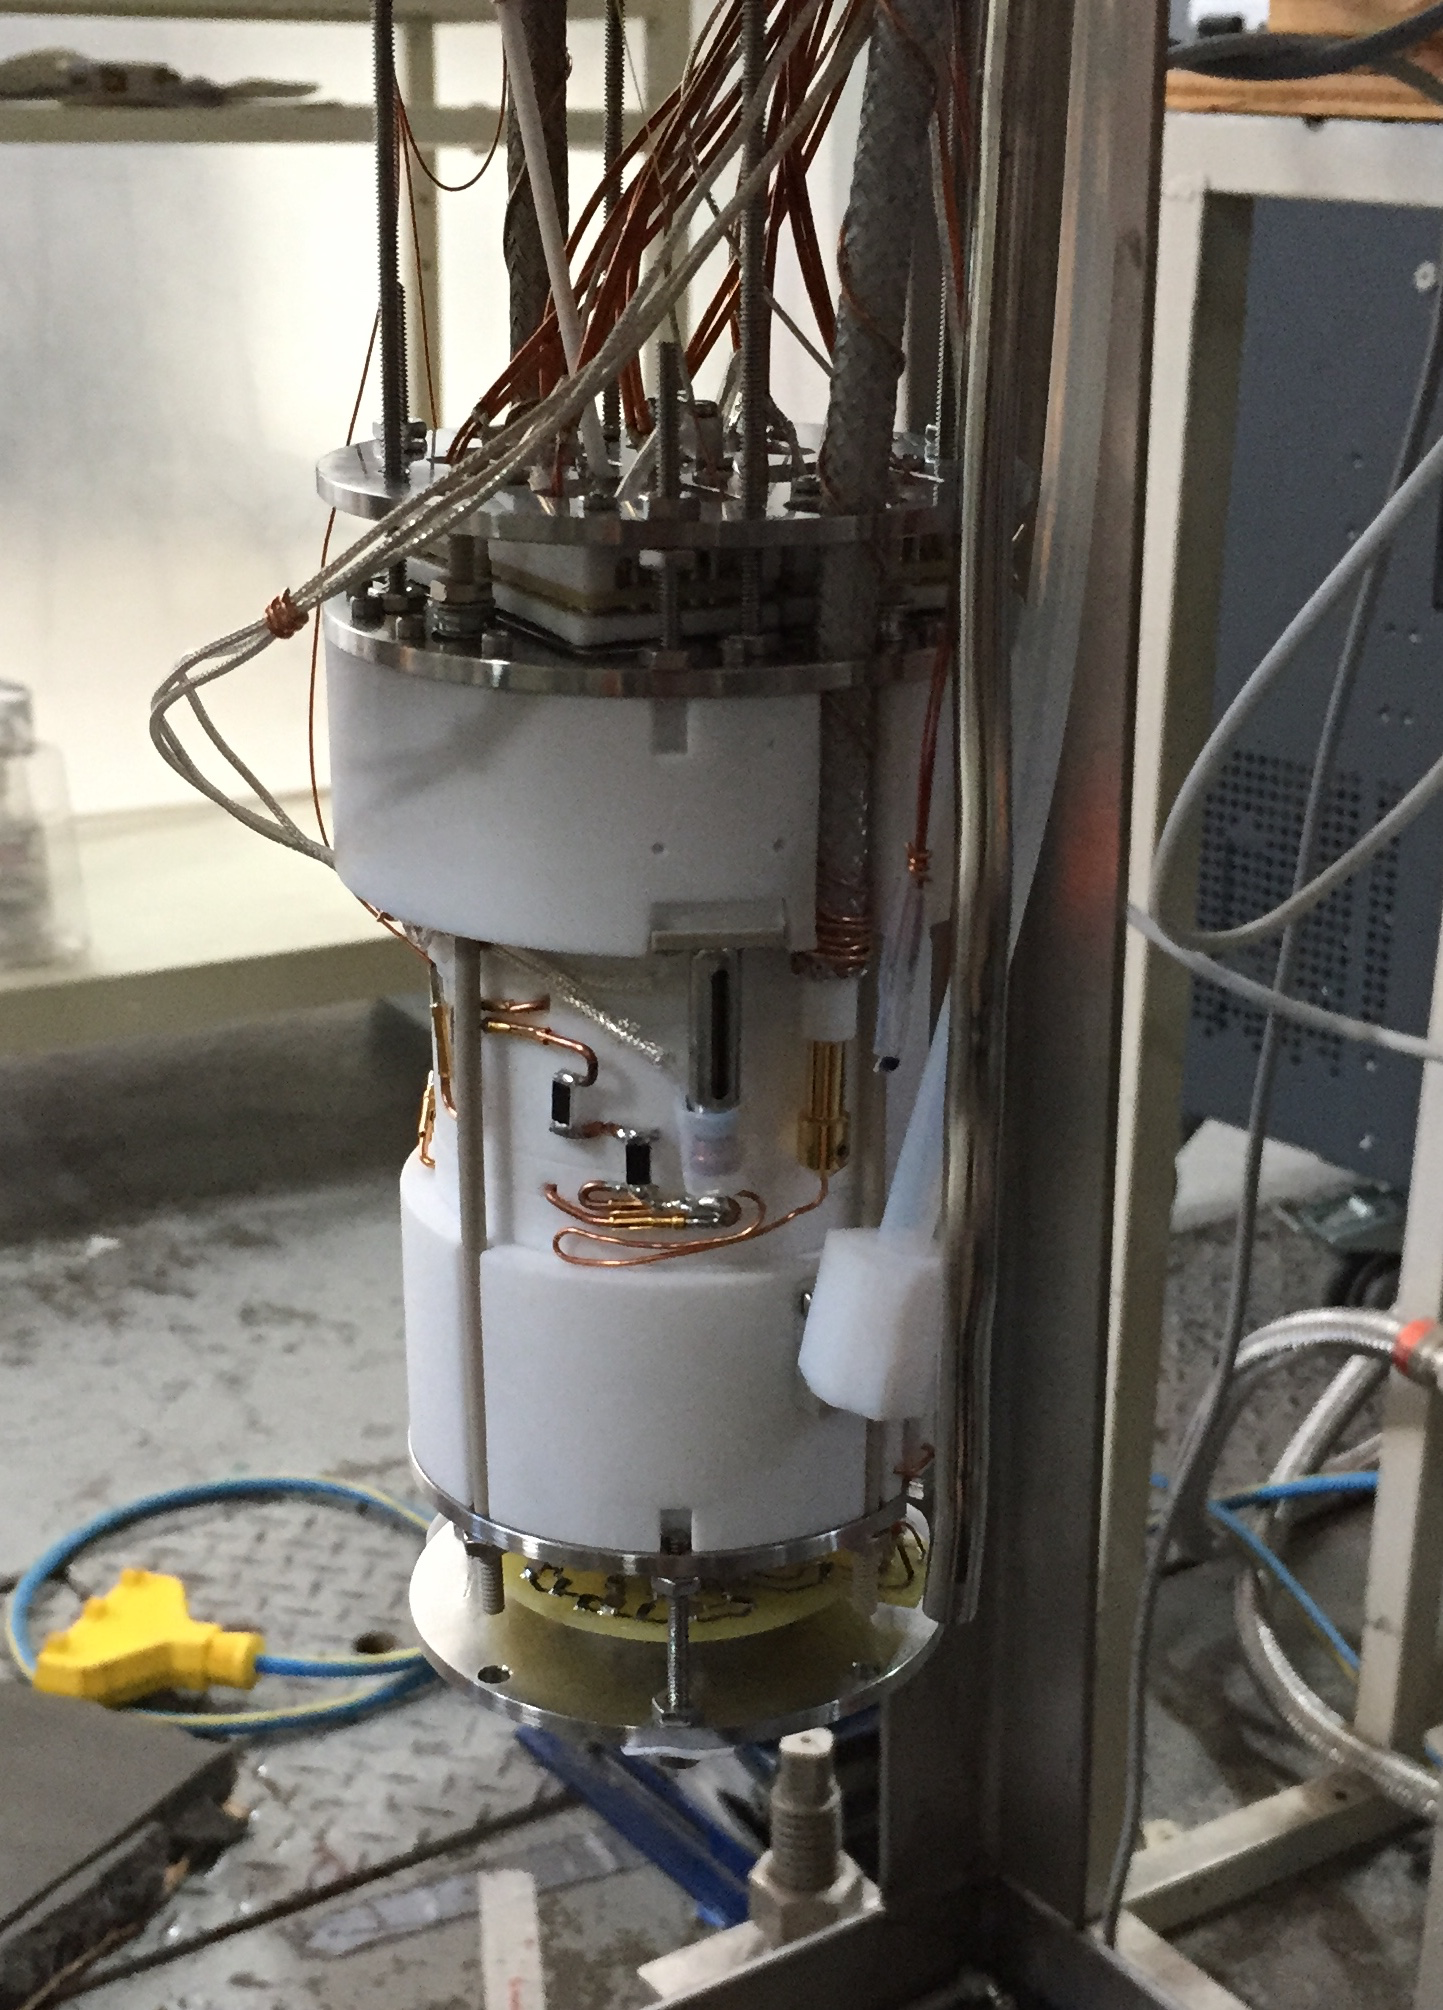
\includegraphics[width=0.48\textwidth]{nerix_tpc_cathode}
	\caption{Two photos of the neriX TPC following routine detector maintenance.  In both photos, one can see the plates holding the single 2'' PMTs (bottom) and the array of four 1'' PMTs (top).  In the left image, one can see the high voltage feedthrough for the anode.  On the right image, one can see the high voltage feedthrough for the cathode and the voltage divider for the field shaping ring.  One can also see the stainless steel pipe used to extract xenon from the inner cryostat's buffer and the plastic tube used to feed re-condensed xenon into the system.}
	\label{fig:nerix_tpc}
\end{figure}



\begin{figure}[t]
        \centering
	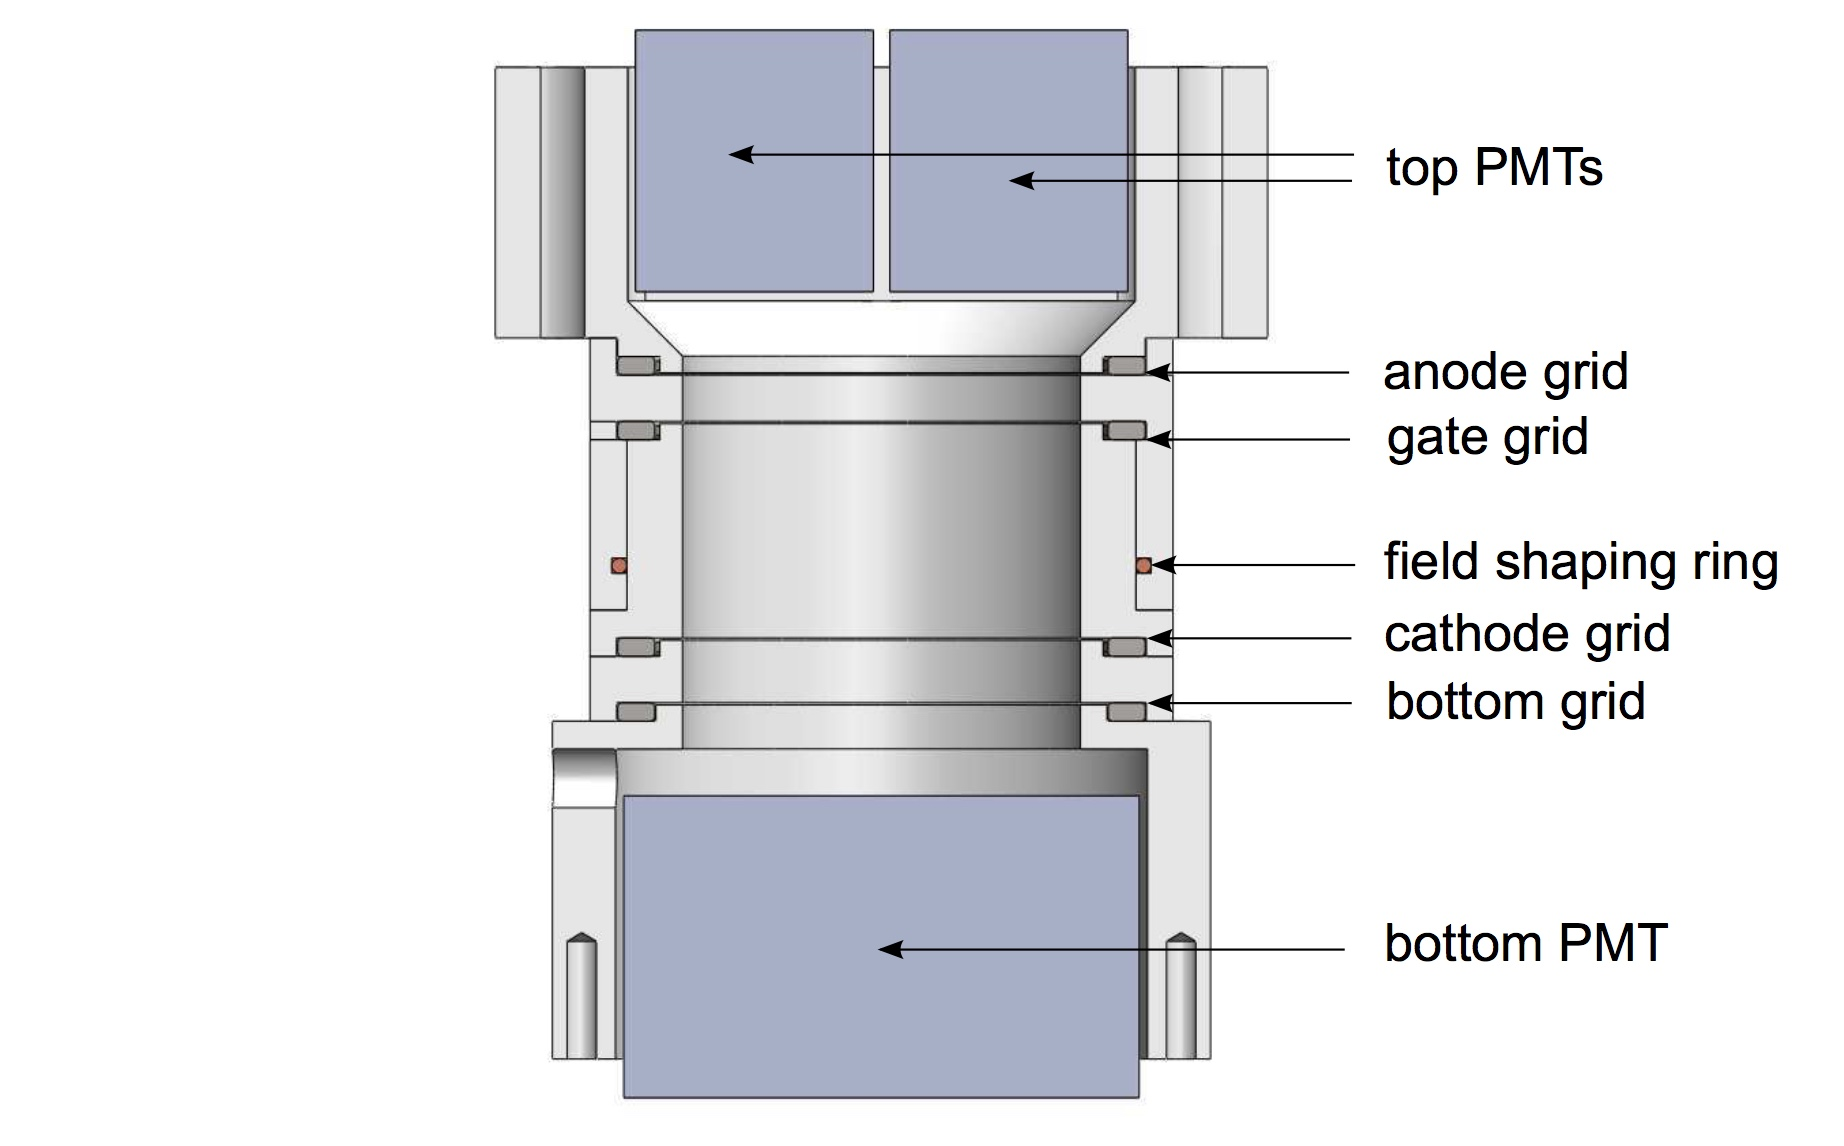
\includegraphics[width=0.8\textwidth]{nerix_tpc_labeled}
	\caption{The neriX TPC with meshes and PMTs labelled.}
	\label{fig:nerix_tpc_labeled}
\end{figure}
   
   
\begin{figure}[bt]
        \centering
	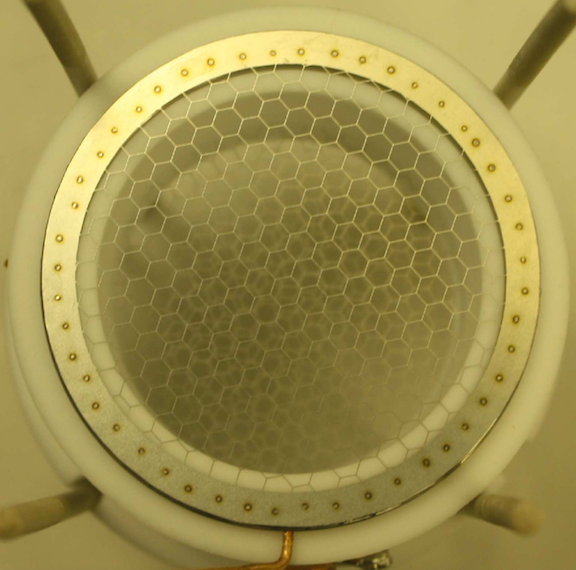
\includegraphics[width=0.5\textwidth]{nerix_tpc_mesh}
	\caption{A photo of one of the meshes used in neriX.}
	\label{fig:nerix_tpc_mesh}
\end{figure}



Six PMTs are installed in neriX: a single 2'' Hamamatsu R6041 PMT is installed below the screening mesh, four 1'' multianode Hamamatsu R8520-M4 PMTs are installed above the anode mesh, and a single 1'' Hamamatsu R8520-406 is installed in a light-tight stainless steel enclosure located above the TPC.  This final PMT is coupled to the TPC via a 1 mm fiber optic cable placed in between the four 1'' PMTs and is intended for measuring the decay times of singlet and triplet states in liquid xenon (although this measurement was not performed during the nuclear recoil calibration).  Since almost all light from the scintillation signal in the LXe is reflected at the liquid-gas interface, the bottom PMT is the only PMT used for measuring S1 and S2 signal size for simplicity leaving the top PMTs used for the position reconstruction of an interaction.

The TPC was connected to the cryostat via a stainless steel motion feedthrough that could be used to raise and lower the detector with a precision of $\sim 25 \, \mu$m.  This motion feedthrough could be used to raise and lower the liquid level relative to the TPC since the liquid level was kept constant via the buffer volume discussed in \secref{sec:nerix_cryostat}.

%The neriX TPC in many ways is very similar to the XENON1T TPC.  Both are made of PTFE (teflon), have meshes to produce


\subsubsection{Cryostat}
\label{sec:nerix_cryostat}

The TPC is surrounded by a double-walled vacuum insulated cryostat.  The inner cryostat was custom made for neriX such that the amount of inactive xenon is minimized.  This inner cryostat, shown in \figref{fig:nerix_cryostat_tpc}, left only approximately 1 cm of space between itself and the TPC with the exception of a $\sim 165 \textrm{cm}^3$ buffer volume used to maintain the liquid level and the space left for the high voltage feedthroughs.   The cryostats themselves are only 1.5 mm thick.  To reduce radiative heat transfer, the inner cryostat is blanketed with mylar in the same way as XENON1T.


\begin{figure}[t]
        \centering
	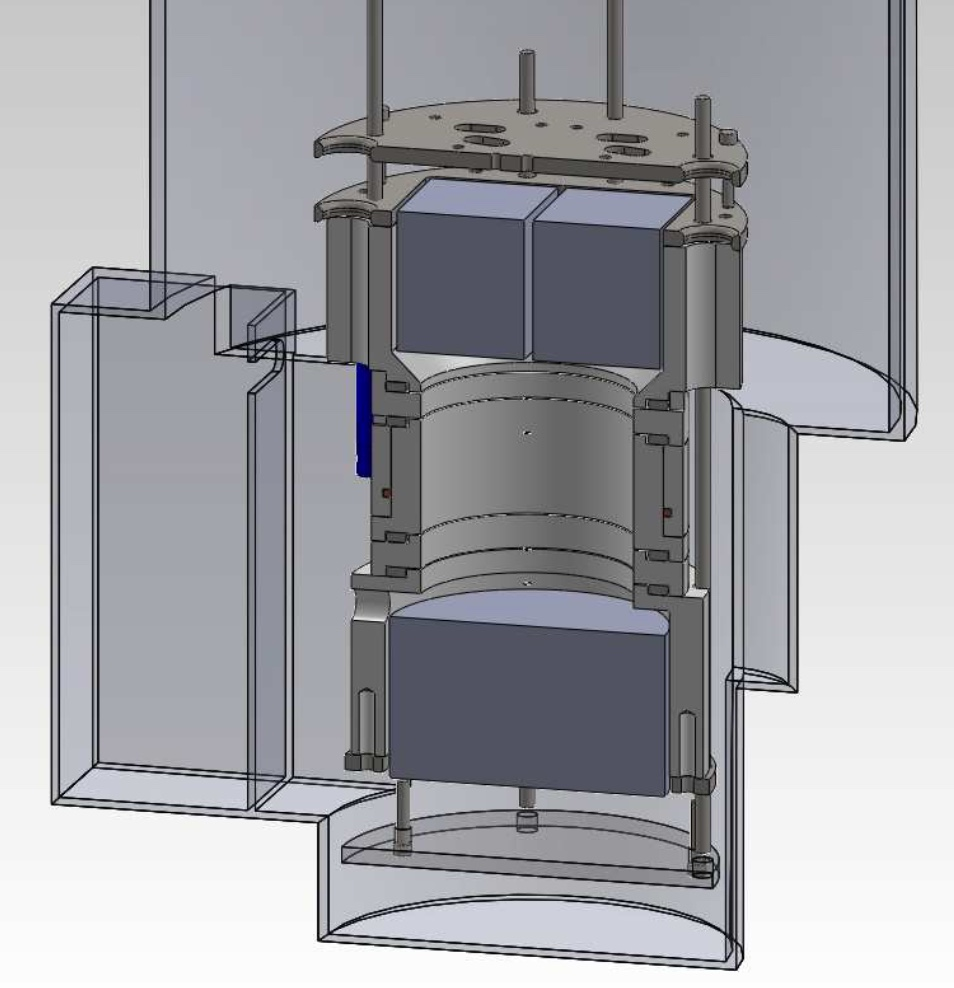
\includegraphics[width=0.5\textwidth]{nerix_cryostat_tpc}
	\caption{The neriX TPC inside of the cryostat.  Note that excluding the buffer volume (left side of the image) and the space left for the high voltage feedthroughs (right side of the image), very little space is left between the cryostat and the TPC, effectively reducing the amount of inactive xenon for undetectable energy losses.}
	\label{fig:nerix_cryostat_tpc}
\end{figure}


\subsubsection{Purification and Cryogenics System}
\label{sec:nerix_cryo_pur}

A diagram of the cryogenics and purification system is shown in \figref{fig:nerix_cryo_pur}.  The cryogenics and purification system used for this measurement is the same as the one used in the measurements of both \citeref{plante2011new} and \citeref{goetzke2016measurement}.

As discussed in earlier chapters, electronegative impurities outgassed from the detector materials will absorb electrons extracted from the interaction site.  Therefore, these impurities must constantly be removed from the xenon to ensure optimal detector operation.  To remove impurities in neriX, the SAES PS4-MT3-R-1 hot getter is used.  Gaseous xenon is flowed through the purification system at approximately 2 SLPM (standard liters per minute) using a KNF N 143 double-diaphragm pump.  A heat exchanger, as described in \citeref{giboni2011xenon}, is used to simultaneously heat up the gaseous xenon coming from the detector and cool down the xenon going towards the detector (from the getter).  This heat exchanger substantially lowers the cooling power required to operate the detector.

To maintain the temperature of the detector, Iwatani PDC08 cold head and SA101 Helium compressor coupled to a copper cold finger are used.  The xenon pressure inside of the cryostat is maintained via resistive heaters thermally connected to the copper cold fingers.  These resistive heaters are controlled by a proportional-integral-derivative (PID) controller that adjusts the power of the heaters to maintain a desired cold-finger temperature.


\begin{figure}[t]
        \centering
	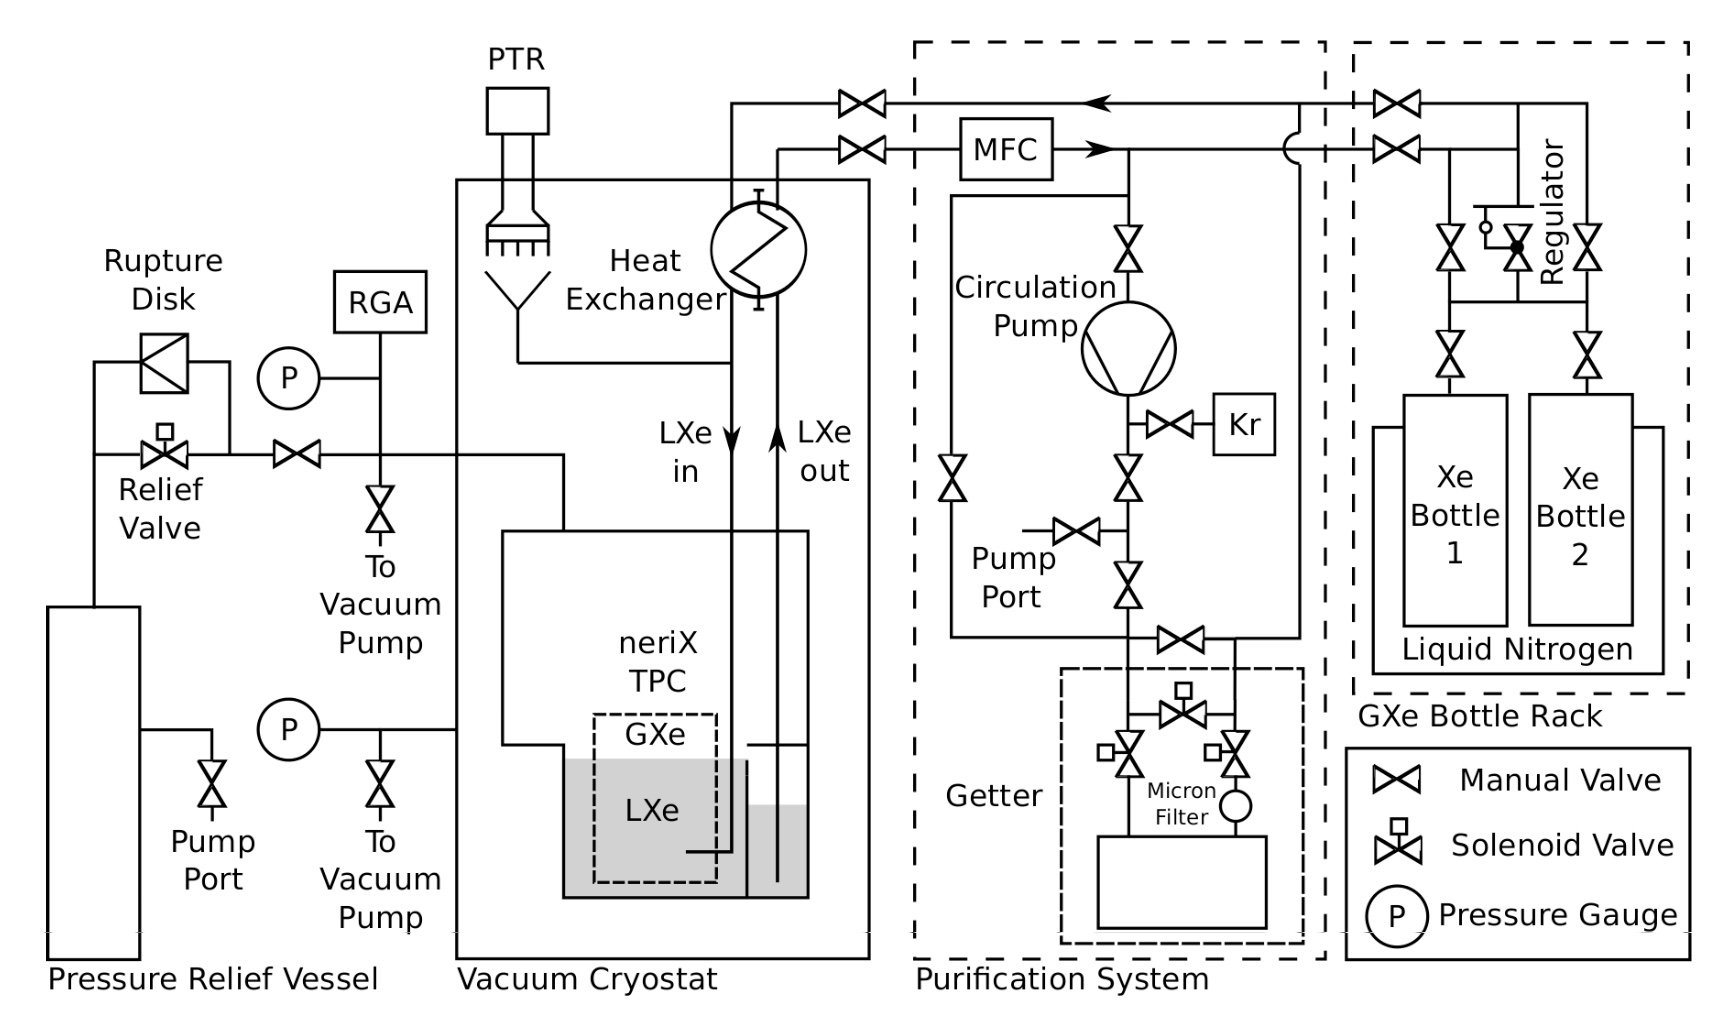
\includegraphics[width=0.99\textwidth]{nerix_cryo_pur}
	\caption{A schematic of the cryogenics and purification system for neriX.  Also shown are the pressure relief system and the xenon storage system.}
	\label{fig:nerix_cryo_pur}
\end{figure}



\subsubsection{Pressure Relief System}

Unlike XENON1T, there is no redundant liquid nitrogen cooling in the event of a power loss for neriX.  This means that if there is a power failure at the laboratory that cooling will be lost and the pressure of the detector will climb.  To prevent damage to the system, especially the PMTs, a pressure relief system was built for neriX.  This pressure relief system consists of a 190 liter stainless steel pressure vessel that is connected to the inner cryostat via a solenoid valve that will open in a controlled manner above a certain pressure in parallel with a rupture disk.  The tank size was chosen such that all of the approximately 2.2 kg of xenon could be stored at room temperature at a pressure below 2.5 bar.  The pressure relief vessel was evacuated on a weekly basis to maintain the chemical purity of the xenon in the case of an emergency.


\subsubsection{Xenon Storage}

The xenon for neriX was stored in two cylinders kept inside of a stainless steel dewar.  When filling the detector, a regulator and a needle valve are used in conjunction with a mass flow meter to keep the detector pressure at reasonable levels.  During recuperation, the dewars are filled with liquid nitrogen such that the xenon inside the bottle freezes and the vapor pressure is low enough to create a cryogenic pump from the cryostat to the storage bottles.  While recuperation can be performed more quickly in an emergency situation, both operations could safely be performed in a single day\footnote{Emptying the detector too quickly could lead to the formation of xenon ice which could damage the bottom PMT so care was always taken to maintain a consistent pressure throughout recuperation in non-emergency situations.}.


\subsubsection{Electric Field Strength and Uniformity}

% ensuring <20\% variation in field to define the fiducial volume

Since the goal of neriX is to measure the light and charge yield of nuclear recoils at different electric fields, it is obviously very important to know what electric field you are measuring the yields for and how uniform it is in the detector.  Unlike in XENON1T, the fiducial volume of neriX is not designed to eliminate background but to exclude regions where the field differs drastically from the mean and where charge can be lost to the wall.  To set the fiducial volume and determine the field strength in neriX, the COMSOL Multiphysics\textsuperscript{\textregistered} Suite was used.  

Simulation details can be found in \citeref{goetzke2015low} but we will present the results of the simulation here.  \tabref{tab:nerix_electric_fields} shows the cathode voltages used along with the corresponding fields given an anode voltage of 4.5 kV, a liquid level 2.5 mm above the gate mesh\footnote{The simulations find that the liquid level has a negligible effect though.}, and the bottom mesh and gate mesh kept at ground.  Simulations found that the variation of field could be kept to within 20\% with a radial cut at approximately 20 cm and cuts in depth at 1 mm below the gate mesh and 0.5 mm above the cathode.  For the nuclear recoil calibration, a more conservative radial cut at 18.25 cm was made.  

\begin{table}[t]
\centering
\def\arraystretch{1.3}
\begin{tabular}{c|ccc}
$\textrm{V}_{\textrm{C}}$ [kV] & -0.345 & -1.054 & -2.356 \\
\hline
$\textrm{E}_{\textrm{D}}$ [kV/cm] & 0.19 & 0.48 & 1.02 \\ 
$\pm 1\sigma$ [kV/cm] & 0.03 & 0.05 & 0.12 \\ 
\end{tabular}
\caption{The different cathode voltages used during the nuclear recoil measurement of neriX and the corresponding electric field strength and field variance.  The simulation assumes an anode voltage of 4.5 kV, a liquid level 2.5 mm above the gate mesh, and the bottom mesh and gate mesh kept at ground.}
\label{tab:nerix_electric_fields}
\end{table}



\subsubsection{Data Acquisition System and Processing}

Raw PMT signals are amplified and then digitized by three CAEN V1724, 14 bit, 100 MS/s flash ADCs (fADC).  The fADC has a voltage range of 2.25 V, and an input bandwidth of 40 MHz.   Three flash ADCs were required to digitize the 18 PMT signals as well as the multiplexed liquid scintillator signals.  The trigger for the data acquisition system used in this measurement will be discussed in \secref{sec:nerix_coin_trigger} and \secref{sec:nerix_pure_trigger}.

The data processing system, xerawdp, was originally developed for XENON100 \cite{guillaume_thesis} and modified for neriX.  The processing software was used to reduce the raw waveforms into information about the S1, S2, and liquid scintillator signal sizes and timing.  




\subsection{Neutron Generator}

As mentioned in \secref{sec:nerix_expt_setup}, a small \ce{^2H}$(d, n)$\ce{^3He} generator, shown with a ruler for scale in \figref{fig:nerix_minitron_ruler},  is used to produce neutrons.  This generator is provided by the Schlumberger Princeton Technology Center and will be referred to in this work as the minitron.  The tube of the generator is vacuum sealed and deuterium is produced inside by heating up a replenisher filament.  These deuterium atoms are then ionized via electrons produced from a cathode wire that are accelerated by a grid kept at $\sim 200$ volts.  Deuterium ions are then accelerated towards a titanium-deuteride (\ce{TiD_2}) target where they will either collide with a deuterium atom or be completely stopped.  Deuterium ions that are completely stopped actually replenish the target and thus the target is considered self-regenerating\footnote{The thickness of the target is such that all deuterium ions are stopped.}.  A Heinzinger PNC 100000-3 power supply is used to supply up -100 kV of voltage to accelerate the deuterium ions and to read out the deuterium ion beam current.  A schematic of the minitron electronics is shown in \figref{fig:nerix_minitron_schematic}.

Because the minitron neutron generator operates at very high voltage, a protective casing was used to prevent disharges from the high voltage connection. The casing was a stainless steel tube with a diameter of approximately 3 inches and teflon, due to its very large dielectric constant, supporting the minitron and filling in almost all excess space in the stainless steel tube.  The small amount of remaining space was filled with mineral oil, which has a higher dielectric constant than air.

The neutron generator used in this work is the same as used in \citeref{plante2011new}.  For more details on the minitron, please refer to \citeref{guillaume_thesis}.


\begin{figure}[t]
        \centering
	\includegraphics[width=0.99\textwidth]{nerix_minitron_ruler}
	\caption{The deuterium-deuterium neutron generator used to produce 2.45 MeV neutrons.}
	\label{fig:nerix_minitron_ruler}
\end{figure}


\begin{figure}[bt]
        \centering
	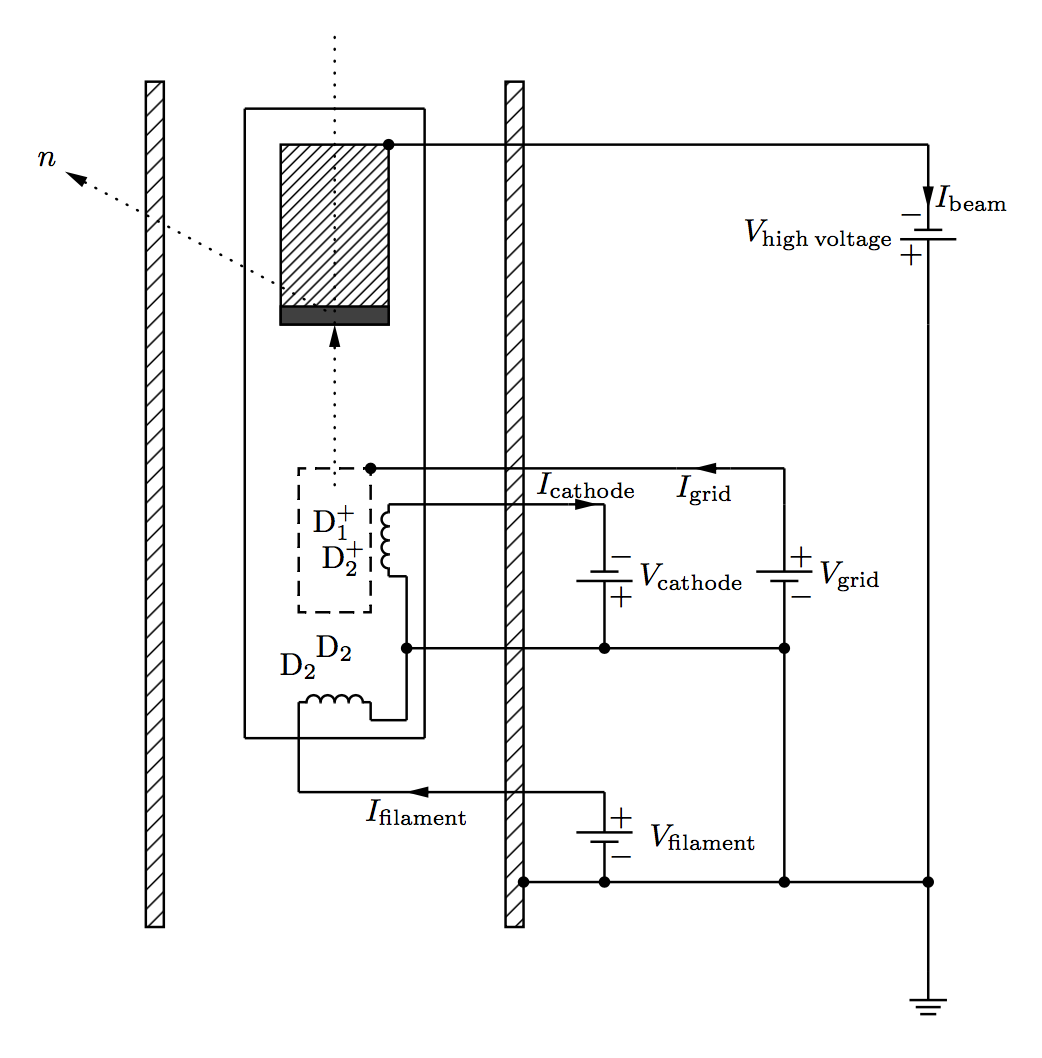
\includegraphics[width=0.65\textwidth]{nerix_minitron_schematic}
	\caption{The electronics of the minitron neutron generator.  Image Credit: \citeref{guillaume_thesis}.}
	\label{fig:nerix_minitron_schematic}
\end{figure}


\begin{figure}[t]
	\centering
	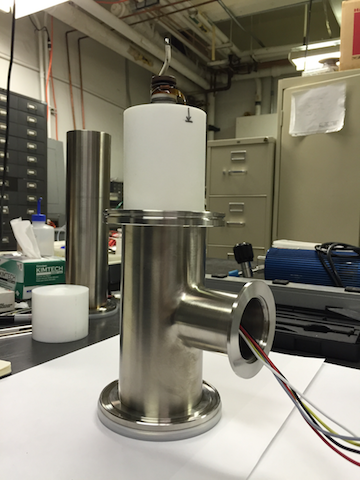
\includegraphics[width=0.533\textwidth]{nerix_minitron_partial_case}
	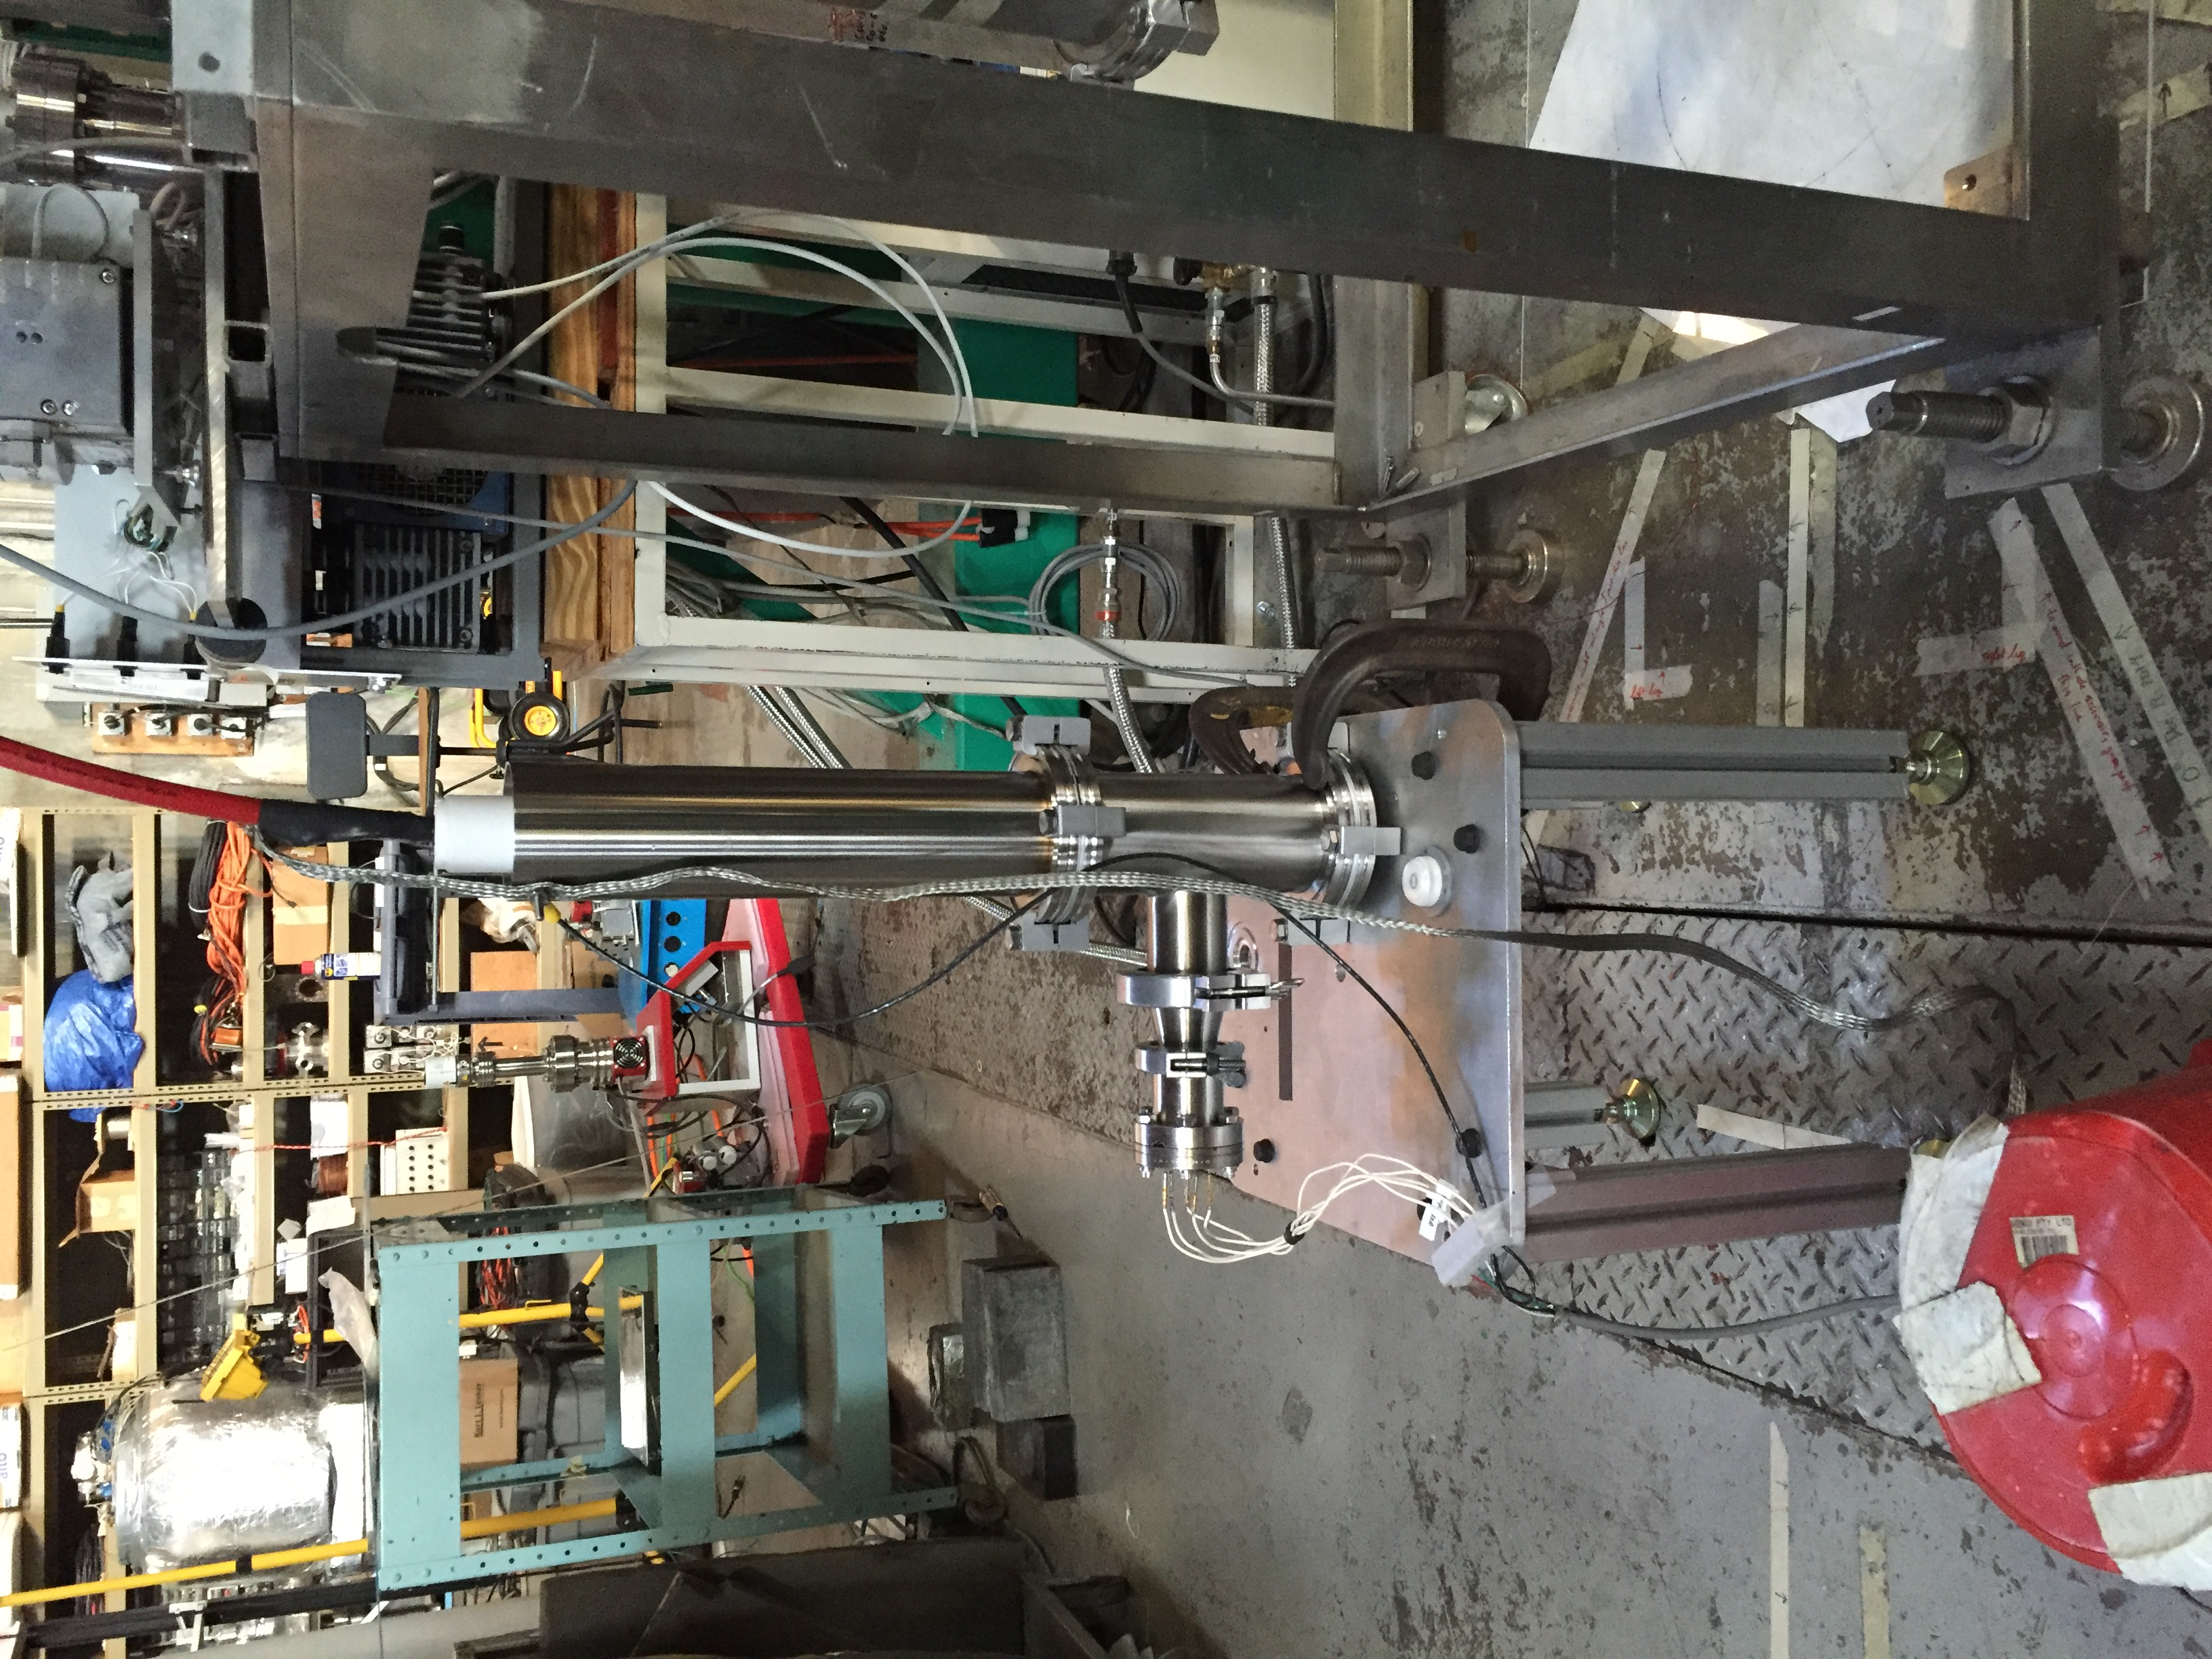
\includegraphics[width=0.4\textwidth]{nerix_minitron_set}
	\caption{On the left, the minitron in its partially constructed case.  Notice that the teflon leaves very little room between the steel and minitron to maximize the potential voltage that can be used without causing an electrical breakdown.  On the right, the minitron in its final set position.  While not visible, the minitron case has been filled with mineral oil at this point to reduce risk of electrical breakdowns.}
	\label{fig:nerix_minitron_rate}
\end{figure}


\subsubsection{Neutron Energy Spectrum}

For non-relativistic deuterons,  the energy of the neutron produced from a deuterium-deuterium interaction is only dependent on the scattering angle and the energy of the deuteron.  The exact energy, in this case, is given by \eqnref{eqn:nerix_neutron_energy} \cite{csikai1987crc}. 

\begin{equation}
        \label{eqn:nerix_neutron_energy}
        abc
\end{equation}

In \eqnref{eqn:nerix_neutron_energy}, $m_{\textrm{He}}$, $m_n$, and $m_d$ are the masses of helium, neutrons, and deuterium, respectively, $Q$ is the $Q$-value of the reaction (3.269 MeV), and $\phi$ is the emission angle of the neutron in the laboratory frame.  To approximate the energy spectrum as a function of the scattering angle and deuteron energy, we say that the yield as a function of these variables is proportional to the differential cross-section multiplied by the distribution of incident deuteron energies, $f(E_d)$\footnote{This derivation of the angular dependence of the neutron energy spectrum is from Qing Lin (current institution: Columbia University)}.  We could assume that this distribution of deuteron energies is a delta function for the fixed target collision but this would ignore all of the other interactions that can occur in the \titde{}.  

\begin{equation}
        \frac{d^2 N}{d E_d d \varphi} \sim \frac{d \sigma}{d \varphi} f(E_d)
\end{equation}

Since the energy of the deuteron is directly related to the energy of the neutron produced by \eqnref{eqn:nerix_neutron_energy}, we can rewrite the above equation in terms of the neutron energy and the emission angle.

\begin{equation}
        \frac{d^2 N}{d E_n d \varphi} \sim \frac{d \sigma}{d \varphi} f(E_d) \left( \frac{\partial E_n}{\partial E_d} \right)^{-1}
\end{equation}

We now define two variables: $\sigma_n$, the total cross-section of deuterium-deuterium fusion into a neutron, and $\sigma_{\textrm{tot}}$, the total cross-section of all possible interactions.  It turns out that $\sigma_{\textrm{tot}} \gg \sigma_n$ due to Rutherford scattering.  Therefore, we say that probability of a neutron being produced per interaction is given by $p = \frac{\sigma_n}{\sigma_{\textrm{tot}}}$.  We say that the number of interactions is approximately given by the energy lost, $E_l$, divided by the average interaction energy, $W$.  We define $W$ in terms of the stopping power such that $W = \frac{dE / dx(E_d) \cdot M}{\sigma_{\textrm{tot}} N_a}$, where $N_a$ is Avogadro's number and $M$ is the molar mass of \titde{}.

Therefore, we approximate the probability that the incoming deuteron, with an energy of $E_{d, m}$, fuses with a deuteron in the target after $i = \frac{E_{d, m}}{W}$ interactions is given by \eqnref{eqn:nerix_minitron_energy_loss_1}.

\begin{equation}
        \label{eqn:nerix_minitron_energy_loss_1}
        f(E_l) \sim \left( 1 - \frac{\sigma_n}{\sigma_{\textrm{tot}}} \right)^i = \left( 1 - \frac{\sigma_n}{\sigma_{\textrm{tot}}} \right)^{E_l \cdot \frac{\sigma_{\textrm{tot}} N_a}{dE / dx(E_d) \cdot M}}
\end{equation}

This expression for the distribution of the energy lost by the incoming deuteron can be rearranged into a more convenient form.

\begin{equation}
        \label{eqn:nerix_minitron_energy_loss_2}
         f(E_l) \sim \left[ \left( 1 - \frac{1}{\frac{\sigma_{\textrm{tot}}}{\sigma_n}} \right)^{\frac{\sigma_{\textrm{tot}}}{\sigma_n}} \right] ^{E_l \cdot \frac{\sigma_n N_a}{dE / dx(E_d) \cdot M}} \approx e^{-E_l \cdot \frac{\sigma_n N_a}{dE / dx(E_d) \cdot M}}
\end{equation}

With an approximate distribution for the energy loss, and therefore the deuteron energy during the fusion interaction, we can simulate our expected angular distribution \cite{chadwick2011endf, guillaume_thesis}.  The angular distribution assuming a maximum deuteron energy of 80 keV is shown in \figref{fig:nerix_yield_emission_angle}.

\begin{figure}[t]
        \centering
	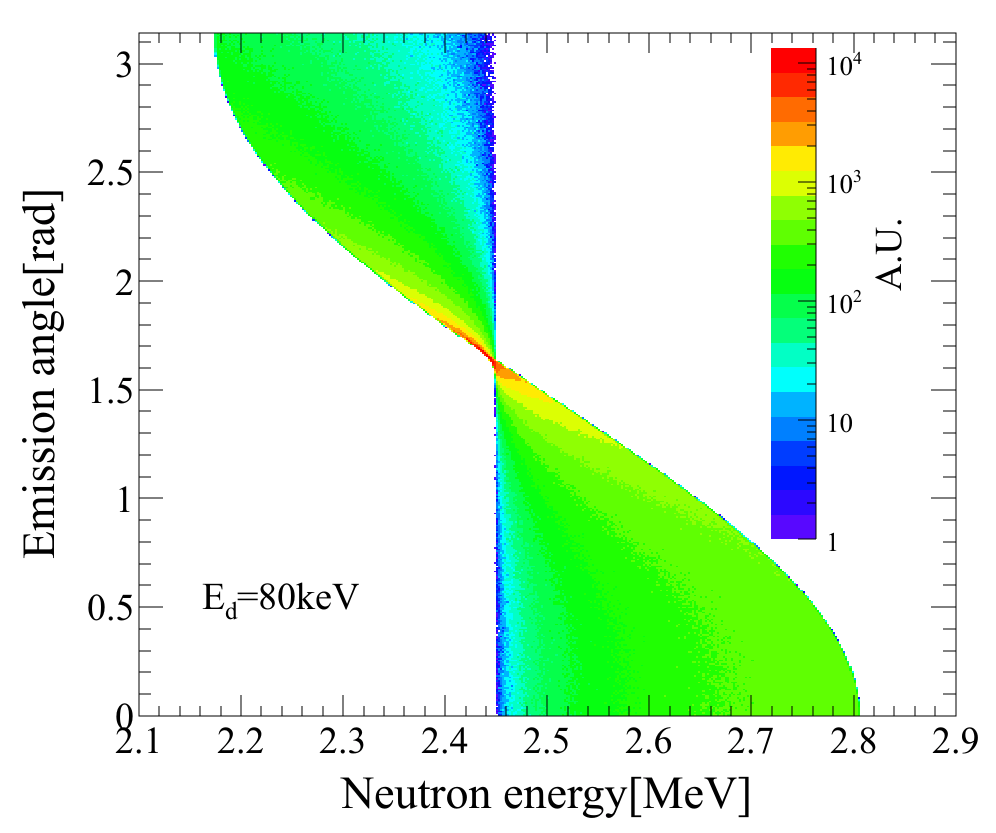
\includegraphics[width=0.75\textwidth]{nerix_yield_emission_angle}
	\caption{The expected angular distribution of neutrons as a function of emission angle for a maximum deuteron energy of 80 keV.}
	\label{fig:nerix_yield_emission_angle}
\end{figure}





\subsubsection{Neutron Yield}

While ultimately we did not include the neutron rate in our analysis of the yields, we did characterize the neutron generator to ensure that it was operating as expected.  \citeref{guillaume_thesis}, following the analysis from \citeref{csikai1987crc}, shows that the flux of neutrons generated should increase approximately exponentially with the high voltage used to accelerate the ionized deuterium atoms and molecules and linearly with the deuterium ion beam current.  We assume that these two effects are uncorrelated and therefore the neutron production rate can be written as $\frac{dN}{dt} = f(I)g(V)$ where $f(I)$ describes the rate's dependence on the beam current and $g(V)$ describes the rate's dependence on the high voltage.

The neutron flux of the minitron neutron generator was measured using a Nuclear Research Corporation NP-2 portable neutron monitor \cite{np2_manual}.  The NP-2 neutron monitor uses a \ce{BF_3} target to create alpha particles which can then ionize the gas in the detector.  The target is housed inside of a polyethylene moderator with a high hydrogen content to increase the detector's efficiency.  The detector measures in units of dose rate which can be converted to flux by means of the fluence per unit dose equivalent of 2.45 MeV neutrons.  As mentioned, we approximated that the current and high voltage could be treated separately and measured the change in one while holding the other fixed to characterize the neutron flux.  For the measurement, the NP-2 detector was placed 180 cm away from the neutron generator (inside of its case) and at an angle of $\frac{\pi}{2}$.  The rate measurements were then used to fit rate as a function of beam current and voltage (shown in \figref{fig:nerix_minitron_fits}).  Using these functions, we can then predict the neutron flux of the minitron, as shown in \figref{fig:nerix_minitron_rate}.

%shielding oil teflon etc

\begin{figure}[p]
	\centering
	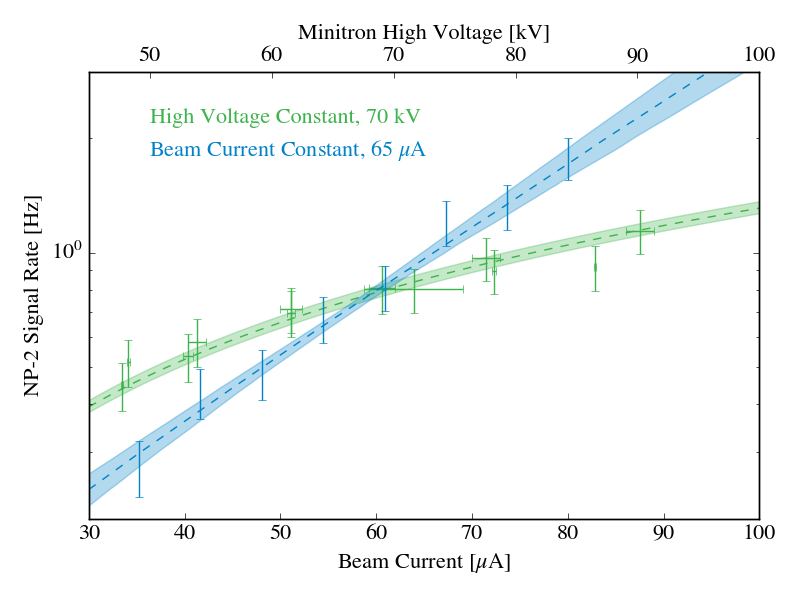
\includegraphics[width=0.8\textwidth]{nerix_minitron_fits}
	\caption{The NP-2 neutron detector signal rate as a function of beam current, holding the high voltage fixed, and high voltage, holding the beam current fixed.  Shaded regions represents 68\% credible region while dotted lines show the best fits.}
	\label{fig:nerix_minitron_fits}

        \vspace{\floatsep}

	\centering
	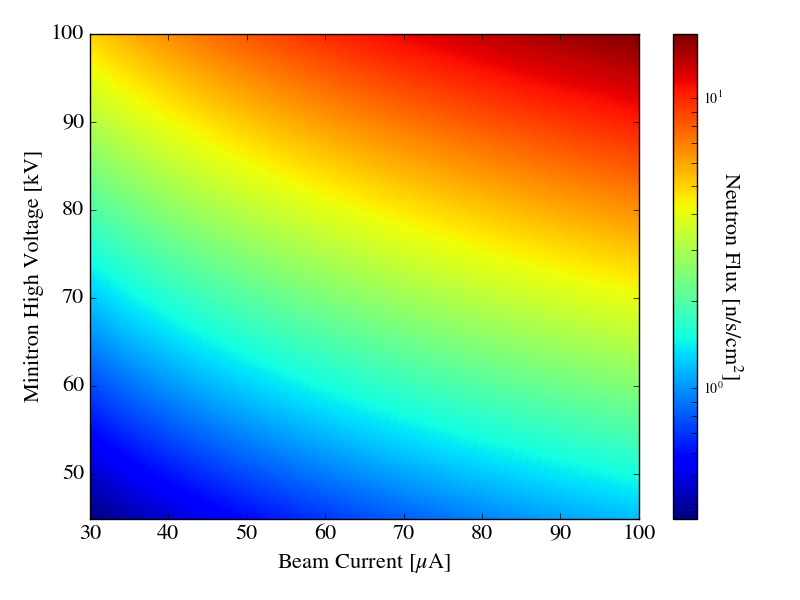
\includegraphics[width=0.8\textwidth]{nerix_minitron_rate}
	\caption{The expected neutron flux from the minitron neutron generator at a distance of 180 cm at an angle of $\frac{pi}{2}$.}
	\label{fig:nerix_minitron_rate}
\end{figure}



\subsection{Liquid Scintillators}

In theory, any detector of ionizing radiation could act as the secondary detector in a nuclear recoil calibration.  In practice, however, the gamma ray background rate is large enough in a laboratory setting that detectors with high levels of discrimination are needed to differentiate neutrons from background in the secondary detector.  

For this measurement, the M510 detectors from Eljen Technologies were used.  The M510 detector is filled with the liquid scintillator EJ301, chosen for its excellent pulse shape discrimination properties.  The EJ301 compound has three characteristic decay times: 3.16, 32.3, and 270 ns \cite{kuchnir1968time, ej301_manual}.  The first two states are related to the excitation of electrons to the singlet and triplet state, respectively, while the slowest decay time is from the fluorescence of the triplet states \cite{lang2017improved}.  Nuclear recoils in the liquid scintillator will exhibit much longer decay times than electronic recoils caused by gamma rays.  

An initial characterization of the liquid scintillators was performed to determine the optimal voltage and integration window for nuclear and electronic recoil discrimination and calibrations were performed several times over the course of the run to ensure performance was still adequate.  An example of the pulse discrimination from one the M510 detectors from coincidence data is shown in \figref{fig:nerix_ej_discrimination}.  Similar to \citeref{guillaume_thesis}, we set a threshold in the detectors' pulse size where discrimination is poor - however this was done via the hardware trigger and not a software cut to reduce data intake. 

\begin{figure}[t]
        \centering
	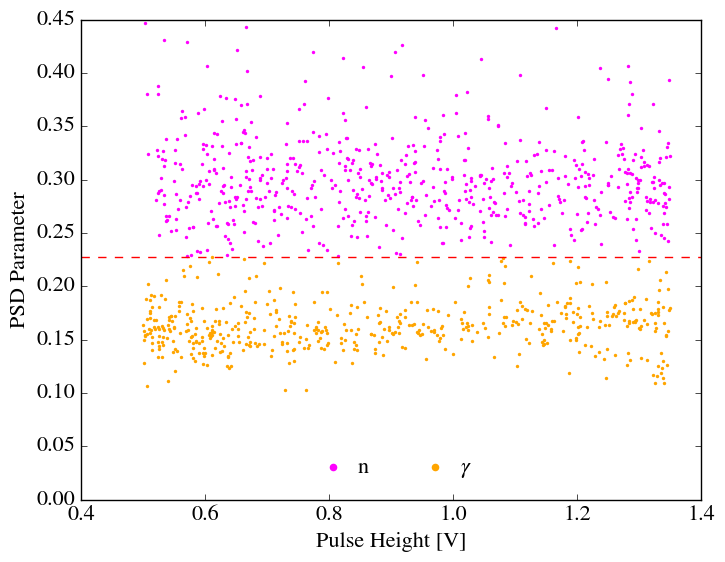
\includegraphics[width=0.75\textwidth]{nerix_coin_ej}
	\caption{Discrimination space for one of the four M510 detectors from coincidence data.  Notice that a hardware cut is made via a threshold discriminator at approximately 500 mV in order to remove events with poor pulse shape discrimination.}
	\label{fig:nerix_ej_discrimination}
\end{figure}

A fifth and smaller version of the M510 detector was placed 180 cm away from the neutron generator to monitor the minitron rate at all times.


\section{Characterization and Calibration of neriX}

As mentioned in chapters two and three, the process from energy deposition to the S1 and S2 signal read out of a waveform for analysis can essentially be broken down into two subsections: the signal production and the detector physics.  If we want to measure the physics of the signal production mechanism, we must be able to decouple the detector physics as well as possible.  To do this, we must make independent measurements to characterize the detector as best as we can.  

While many of the properties of the detector we are trying to characterize are the same as XENON1T, there are some differences in how we carry out the measurements simply due to the scale of XENON1T relative to neriX.



\subsection{PMT Characterization}

As in XENON1T, the most basic task in characterizing the TPC is the PMT calibration.  The goal of the PMT calibration is to understand the response of a PMT to incident photons.  This task is typically performed by examining the response of the PMT to a single photoelectron (single electron ejected at the photocathode by incident photon) since larger signals can be estimated via the convolution of multiple single photoelectron response functions.  Ideally, we would like to completely understand the shape of the response function of the PMT but at the same time, most experiments settle for the mean and variance of the response (since by the central limit theorem these will describe the response for large numbers of photons).  However, since we wish to understand the low energy response of nuclear recoils, which will involve very small signals ($< 10$ PE), we cannot settle for knowing only the mean and variance.

As in XENON1T, the low light calibration of PMTs is performed \textit{in situ} using a blue LED pulse generated by digital pulse generator (BNC PB-5) and fed into the detector via a fiber optic cable.  The standard way of calibrating a PMT in this type of experiment is to use a low light level (such that the given PMT only sees a signal 5--10\% of the time) and either fit the data using a Gaussian model of the response or extract the mean and variance according to the statistical treatment in \citeref{saldanha2017model}.  However, neither of these was satisfactory: the former was not satisfactory as it resulted in an unphysical signal for the PMT response approximately 15\% of the time (since the Gaussian distribution is not bounded below by zero) and the latter was not satisfactory given that we are measuring few photoelectron signals and therefore the mean and variance are simply not enough.  Therefore, a new model was developed by the author, called the \textit{cascade model}, which tries to simulate the actual physics of a PMT including the underamplification of electrons and its dynode structure \cite{anthony2017characterization}.  This model is discussed in further detail in \appref{app:pmts} and uses a GPU-based analysis framework, like measurement of the light and charge yield in neriX (the focus of this chapter) and the electronic and nuclear recoil calibration of XENON1T (discussed in \secref{sec:xe1t_er_nr_calibration}), that will be discussed in \appref{app:gpus}.  Unlike the other two calibration methods, it is actually more effective to use a higher light level such that 1--2 photoelectrons are seen on average\footnote{This does not affect the assumption that the number of photoelectrons seen follows a Poisson distribution that is standard in these types of measurements}.  A sample low-light spectrum is shown in \figref{fig:nerix_pmt_best_fit} along with the best fits and 68\% credible regions of both the Gaussian and cascade models.  From this spectrum alone, it does not appear that the cascade model is an improvement but if one looks at \figref{fig:nerix_spe_response}, which shows the full-amplification SPE spectrum for both models, one can see the reason why the Gaussian model is not acceptable: it results in a negative signal a non-negligible fraction of the time.


\begin{figure}[p]
	\centering
	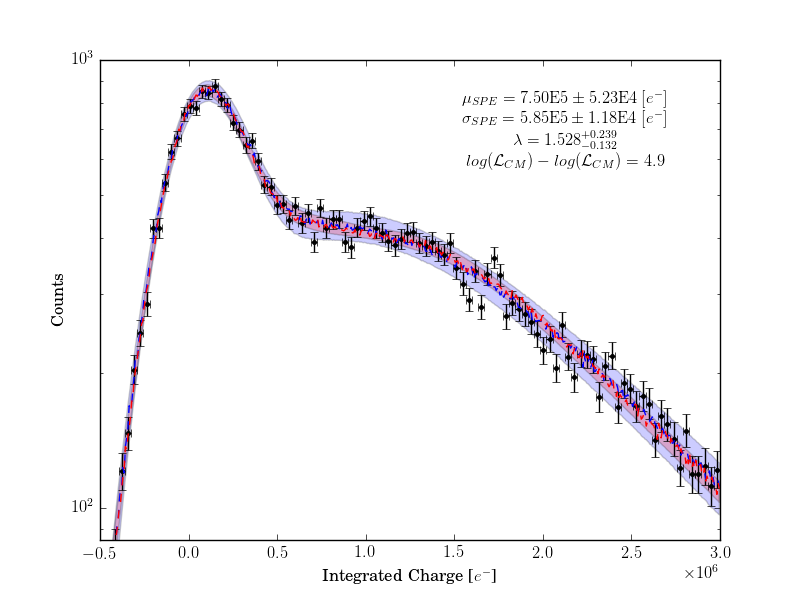
\includegraphics[width=0.8\textwidth]{nerix_pmt_best_fit}
	\caption{.}
	\label{fig:nerix_pmt_best_fit}

        \vspace{\floatsep}

	\centering
	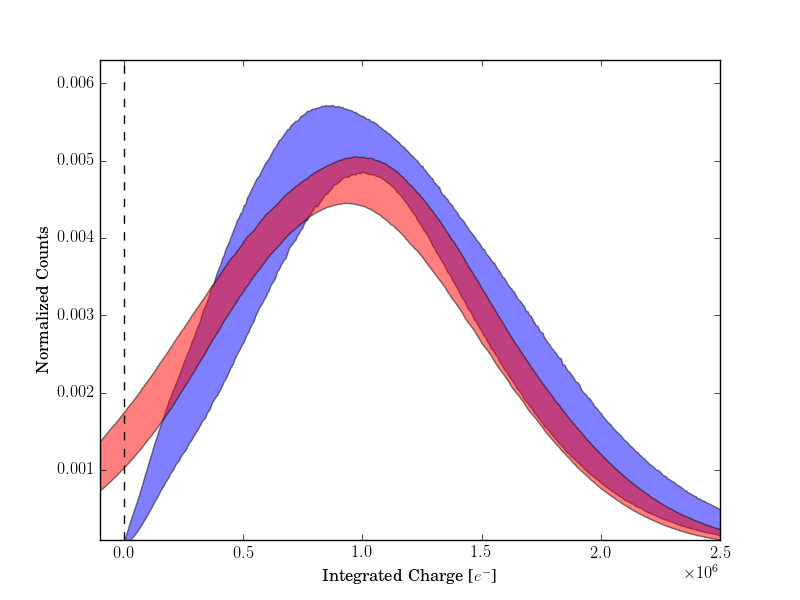
\includegraphics[width=0.8\textwidth]{nerix_spe_response}
	\caption{.}
	\label{fig:nerix_spe_response}
\end{figure}


Unlike \citeref{goetzke2016measurement}, no gain instability was seen during the measurement of the nuclear recoil yields.


\subsection{Position Reconstruction and Position Dependence}

Position reconstruction also plays an important role in neriX.  While position reconstruction is not used to remove background events, fiducial volumes are still set to avoid edge effects from field non-uniformity and electrons capturing on the teflon.  Additionally, we do expect a small amount of position dependence for both the S1 and S2.  

To determine the transverse position of the event, we again use the S2 signal seen by the top PMTs.  




\section{Nuclear Recoil Data Collection}

% trigger info and plot

\section{Analysis of Nuclear Recoils in Liquid Xenon}


\section{Discussion}



